% interactapasample.tex
% v1.05 - August 2017

\documentclass[]{interact}

\usepackage[natbibapa,nodoi]{apacite}
\setlength\bibhang{12pt}
\renewcommand\bibliographytypesize{\fontsize{10}{12}\selectfont}

\usepackage{epstopdf}% To incorporate .eps illustrations using PDFLaTeX, etc.
\usepackage[caption=false]{subfig}% Support for small, `sub' figures and tables
%\usepackage[nolists,tablesfirst]{endfloat}% To `separate' figures and tables from text if required
%\usepackage[doublespacing]{setspace}% To produce a `double spaced' document if required
%\setlength\parindent{24pt}% To increase paragraph indentation when line spacing is doubled

\usepackage[longnamesfirst,sort]{natbib}% Citation support using natbib.sty
\bibpunct[,]{(}{)}{;}{a}{,}{,}% Citation support using natbib.sty
\renewcommand\bibfont{\fontsize{10}{12}\selectfont}% To set the list of references in 10 point font using natbib.sty

%\usepackage[natbibapa,nodoi]{apacite}% Citation support using apacite.sty. Commands using natbib.sty MUST be deactivated first!
%\setlength\bibhang{12pt}% To set the indentation in the list of references using apacite.sty. Commands using natbib.sty MUST be deactivated first!
%\renewcommand\bibliographytypesize{\fontsize{10}{12}\selectfont}% To set the list of references in 10 point font using apacite.sty. Commands using natbib.sty MUST be deactivated first!

\theoremstyle{plain}% Theorem-like structures provided by amsthm.sty
\newtheorem{theorem}{Theorem}[section]
\newtheorem{lemma}[theorem]{Lemma}
\newtheorem{corollary}[theorem]{Corollary}
\newtheorem{proposition}[theorem]{Proposition}

\theoremstyle{definition}
\newtheorem{definition}[theorem]{Definition}
\newtheorem{example}[theorem]{Example}

\theoremstyle{remark}
\newtheorem{remark}{Remark}
\newtheorem{notation}{Notation}

\begin{document}

\begin{titlepage}
  \begin{center}
    \vspace*{1cm}

    \Huge
    \textbf{IoT Control for Carbon Savings}
    \vspace{0.5cm}

    \vspace{0.5cm}
    \LARGE
    User Interface Construction - Assignment 4
    Individual Part


    \vspace{1.5cm}

    \textbf{Ferdinand Wittmann - 100493643}

    \vfill

    \begin{figure}[h]
      \centering
      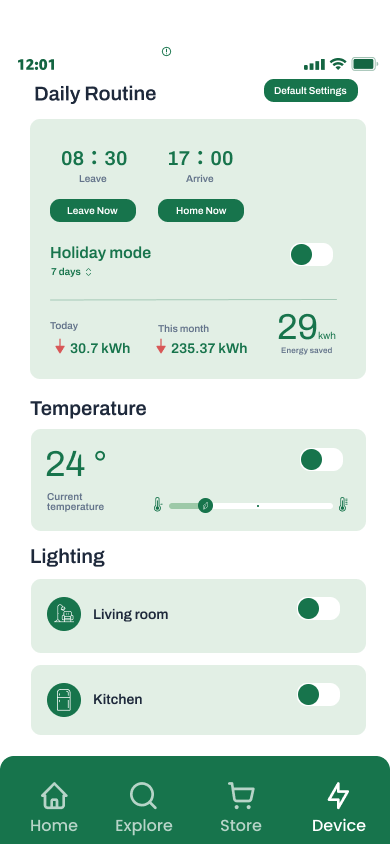
\includegraphics[width=0.3\columnwidth]{img/Screen.png}
      \label{fig:Error}
    \end{figure}

    \vspace{0.8cm}
    \Large
    Department of Computer Science\\
    University of Aalto\\
    Finland\\
    \today

  \end{center}
\end{titlepage}

\section*{Introduction}

\subsection*{Background}

With our world moving towards a more sustainable future, with the goal to successfully stop human-made climate change, we experience a rise in the awareness of ones carbon footprint.
The carbon footprint is the cumulative carbon emissions produced by a persons actions and their consumption \citep*{mulvaney_what_2022}.
Another rising trend is the further integration of Internet of Things Devices (IoT) into households.
It is expected that smart small appliances will almost triple until 2027 \citep*{armstrong_infographic_2022}.
IoT devices are small devices connected to the Internet that can provide value to users through sensor data and by controlling devices that were previously not connected to the internet.
A straightforward application of IoT is controlling the energy consumption of a building.
Learnheat a company focused on saving energy in households by using IoT has shown that they are able to save around 10\% of total energy consumption from consumers \citep*{noauthor_iot_2019}.
In the context of this project, we will explore how we can use user input to further minimize energy usage in households.
The idea is to create a graphical user interface for mobile device, that daily collects information about when users are home and optimizes the heating, AC and lightning of their homes.

\subsection*{User Needs and Goals}

On the one hand many tenants, spend most of their daily activities at their workplace, friends or on holidays.
On the other hand heating system are generally turned on in the winter and then target a specific temperature in the room for night and day, not taking into account if the tenant is actually home.
Even worse are old heating system, that are solely based on the position of a valve that controls the heating system.
A common heater functionality is to have a holiday mode for, which will lower the temperature for set periods of times, controlled by the user.
With energy prices becoming more unpredictable and being a substantial part of a persons spending, while also impacting the persons carbon footprint, there is a need for more optimized heating control.
The goal is to have a IoT device which controls the heating from a household.
On our mobile app the tenant inputs data about when he is leaving his home and when he is arriving again.
The Chatbot then controls the heating unit in an optimal way to save energy, while ensuring that the tenants home is always heated, when he is actually home.
Additionally, the app can control the AC unit in warm regions and the data can automatically turn of lights if the user is not home.
The target customer are households of 1-2 people, because we can assume that in such households the home is not occupied for substantial parts of the day.
The target customer can be well described through the use of personas.
\section*{Methods}
\subsection*{Personas}

Personas are an interaction design technique, that describes target customers through the use of a persona, which is a stereotypical user \citep*{pruitt_personas_2003}.
\citeauthor*{pruitt_personas_2003} analyzed that personas help development teams, because they create a common understanding of the customer and team members can refer to the personas to better communicate their ideas or findings.
Furthermore, personas help the designers towards focusing on human-centered design.
We have identified two personas for our IoT driven and CLI based personal heating control system.

\subsubsection*{Max}

Max is a 24-year-old student, who is currently single. Max lives by himself in an old apartment outside the city.
Max is supported by his parents and tries to save money by eating at the university. Generally, he spends his times studying, meeting friends or going into the city for entertainment.
Max is a digital native and never leaves the house without his smartphone.

Max's Goals:
\begin{itemize}
  \item Wants his room to be warm, when he gets home.
  \item Reducing his carbon emissions
  \item Knowing his carbon emissions
\end{itemize}

Max's Pain Points:
\begin{itemize}
  \item Spend little time configuring his heating system
  \item High costs for heating during the winter
\end{itemize}

\subsubsection*{Patricia}

Patricia is a 29-year-old painter, who is in a new relationship. Patricia lives in the city and bikes to her Atelier, which takes around 30 minutes.
Patricia is highly aware of her carbon footprint and is already shopping carbon aware and values recycling. Patricia spends the morning and afternoons at her work and at night will either go home or sleep at her boyfriends. Patricia uses her mobile phone for connecting with friends, but tries to not use it during work.

Patricia's Goals:
\begin{itemize}
  \item Wants to reduce her carbon emissions as much as possible
  \item Wants to collect data about her carbon emissions
  \item Wants to spend only limited amount of time on her phone
\end{itemize}

Patricia's Pain Points:
\begin{itemize}
  \item She knows that she is spending a lot of time away from her house, but she can not actively control her heating
  \item It is hard for her to track her emissions around multiple different interfaces
\end{itemize}

\section*{Scenario}

The personas give us insights into the user context of use. In the next step we want to create a scenario. A scenario can be useful tool for user interface construction as it describes an application through the lens of an actual user and describes the users' environment.

A user leaves his house to go to work. On the way the user wants to check on his CO2 consumption. The application shows him his carbon footprint and what it consists off. The user then sees that his default setting is set to coming home after 5pm, which is his usual work routine. Today the user actually knows he is spending more time at work and changes the daily setting to coming home after 7pm. During his work day, he forgets what setting he set and rechecks his phone, where he can see his current home coming time.

In the next step we will derive Essential use cases, which are a tool that describe the user intentions and the system requirements.
By defining such, we can ensure that our developed system will reflect the user intentions \citep*{constantine_structure_2000}.
For a more complex application I would suggest going one step further and start doing an object-oriented scenario analysis. This approach is useful tool derive a UML from the scenario, that leads to a common understanding between designer and developer.



\subsection*{Essential Use Cases}

From our personas, our user goals and needs and the scenario we can then derive the essential use cases of our application \citep*{constantine_structure_2000}.
The app can inform the users of their carbon footprint and handprint.
The carbon handprint is calculated from the savings the user achieves by entering the time when their home is unoccupied and the heating is reduced and lightning is turned off.
Furthermore, the app needs to be able to react to changes in the plan of the user.
In summary, we derived the following essential use cases (I: Intention, SR: System Requirement).
\begin{itemize}
  \item I: Display daily carbon footprint; SR: calculate carbon footprint
  \item I: Display carbon savings by use of the app; SR: calculated carbon saving from IoT control
  \item I: Display the current active plan for the IoT control; SR:retrieve the plan
  \item I: Enter time the user leaves the house; SR: update the leaving time in the plan
  \item I: Enter time the user enters the house again; SR: update the arrival time in the plan
  \item I: Change default settings for leaving or entering the house; SR: store a default plan and make it changeable
  \item I: Estimate costs of energy; SR: calculate savings
  \item I: Estimate savings in energy costs; SR: calculate carbon savings
\end{itemize}
For the interface construction we ordered the Tasks in Data Entry and Data Display (the sections are derived from \citeauthor*{smith_guidelines_1986} \citep*{smith_guidelines_1986}).

\begin{itemize}
  \item Data Display: Display daily carbon footprint
  \item Data Display: Display carbon savings achieved from the scheduling of the time spend at home
  \item Data Display: Display the current active plan for the IoT control
  \item Data Entry: Enter time the user leaves the house
  \item Data Entry: Enter time the user enters the house again
  \item Data Entry: Change time default settings for leaving or entering the house
  \item Data Display: Estimate costs of energy
  \item Data Display: Estimate savings in energy costs
\end{itemize}

Here it is interesting to note, that the derived user tasks do not differ between AC and Heating. We will use this for the interface design, where a single temperature control is enough for both AC and Heating, reducing clutter on the interface.

\section*{Results}

\subsection*{Device}

In order to create the best fitting user interface I chose a mobile application. A mobile application fits to our personas and target customers. Their Goal is to make use of the IoT smart devices to control their household energy consumption, while they are not home. Our target users have access to a mobile device and can on-the-go check the status of the system. In order to design the graphical user interface for the application, we will first summarize the tasks and then go in depth into the different screen designs.

\subsection*{Screen Design}

My task was to create the devices Screen, where users can change their settings for arriving and leaving at the house. This also meant changing the default settings for arriving and leaving the house. The data display tasks for the carbon footprint and handprint will be summarized on another Screen designed by another team member. Furthermore, we decided to focus on the implementation of showcasing carbon emissions to create a simpler user interface. In a future version, the estimated monetary savings could be added.

\subsection*{Devices and Default Screen}

The devices screen can be seen in figure \ref{fig:Screen}. Here we applied Gestalt's rules for the visual design \citep*{gkogka_gestalt_2018}.
\begin{itemize}
  \item Proximity: Elements close together are interpreted as one Element
  \item Closure: Elements are supposed to be visually grouped into Boxes
  \item Continuation: Elements are grouped together into one collective elements by finalized design into larger groups like one paper
  \item Simplicity: Ambiguity is interpreted with the easiest interpretation
\end{itemize}




We applied the principle of Continuation by combining all the IoT tasks into one screen and all the default settings onto another Screen (figure 2). The Proximity principle is applied by grouping Temperature, Lightning and Daily Routine into one group. Each group has a title, followed by a visually separated box in green, that groups the data inputs. The grouping helps the user to quickly interpret which elements fit together in order to allow only one interpretation. This design is similarly applied to the Default Screen.

Lastly we want to analyze the user interface design with Nielsen's user interface principles \citep*{nielsen_10_2020}.

\subsubsection*{Visibility of system status}

The system status is displayed at the top of the page, where the users are informed about their daily routine. The daily routine showcases when users leave the house and when they arrive back. In the temperature section users see what target temperature is set for the house and in the lightning section the users see, which lights are currently turned on. We used switches in every section to indicate if a specific IoT control is currently turned on.
Lastly, the current carbon savings are displayed, indicating through an upwards or downwards arrow, if the users is currently saving energy.

\subsubsection*{Match between system and the real world}

In order to match the system state with the users' language we tried to use simple language and icons for better understanding. In the lighting section each element contains an icon for the specific room. The temperature is shown largely in celsius and a thermostat further specifies the grouping.
The wording is chosen in such a way that no miss-interpretation can happen.


\subsubsection*{User control and freedom}

We follow common user interface designs to allow the user to directly understand the interaction. In the default screen an arrow indicates how to leave the settings and is consistent with other mobile application designs.

\subsubsection*{Consistency and standards}

We achieved a consistend user interface, by using design elements commonly used in mobile applications. All the design elements are designed to match the material user interface (MUI) \citep*{noauthor_about_nodate}. MUI has over 4 million weekly downloads and users are likely to know the design elements. Here we are referring to the data input fields for the time and date, the slider and the switches.

\subsubsection*{Error prevention}

The goal for error prevention, was to have a clear and understandable design. I believe we achieved a design that can easily be understood and prevents the user from making mistakes. Furthermore, the leaving now and arriving now button, give the user a shortcut to directly change the settings to reflect his current state. This is the most important information for the user and being able to easily adapt it, helps the user to recover from mistakes.


\subsubsection*{Recognition rather than recall}

Every information users need is clearly visible in one screen. The daily routine, which is the most important user information is positioned at the very top and will directly update, when the user changes his settings.
The user can quickly get the systems state, by scanning the features, which visually present the system state.


\subsubsection*{Flexibility and efficiency of use}

A new user will initially not set his default settings, but if he gets more familiar with the application, the default settings are a great option to enhance his user experience. The default settings set the daily routine based on an earlier user input and save the user time the next time he uses the application.

\subsubsection*{Aesthetic and minimalist design}

One way I reduced the information load was by deciding not to differ between heating and AC and solely control both elements over the temperature setting. Aesthetically I decided on a clear coloring scheme, that highlights important information, and I eliminated all redundant information. I decided to not present the default settings on the devices screen, because they are meant for more familiar users and a familiar users would see that every day his daily routine is updated from the default settings, which would then be redundant information.

\subsubsection*{Help users recognize, diagnose, and recover from errors}

The designed interface does not allow for errors, that lead to an error message. If a user changes a switch by accident, he can easily undo the action. The input for the time is based on a pop-up with a clock, where the user can directly see the new time and update it if a mistake has been made. Additionally, we added the leave now and arrive now button, which help the user to quickly recover from an error. The most important information for the user is if current settings are set for him being home or on the go, as this impacts if the heating will be on or off. By using the update now buttons the user can immediately update this information.


\subsubsection*{Help and documentation}

In order for the user interface to better guide the user, in a future design we would add an information button for each section. This follows other application, who position an information icon next to the header. I believe that this small update to the UI could greatly benefit in guiding the user.


\begin{figure}[h]
  \centering
  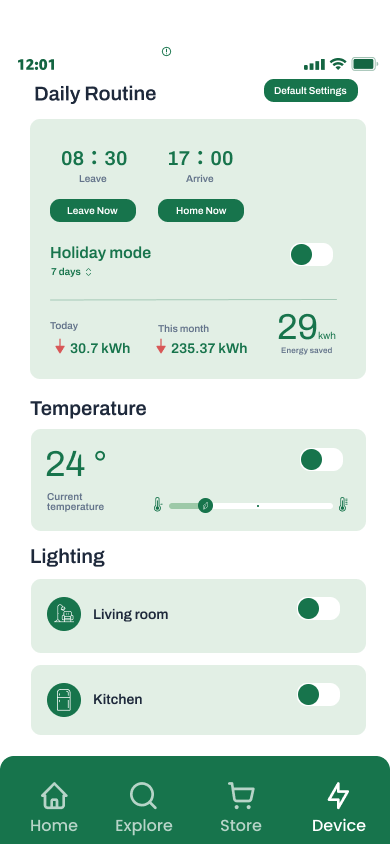
\includegraphics[width=0.3\columnwidth]{img/Screen.png}
  \label{fig:Screen}
  \caption{Devices Screen}
\end{figure}

\begin{figure}[h]
  \centering
  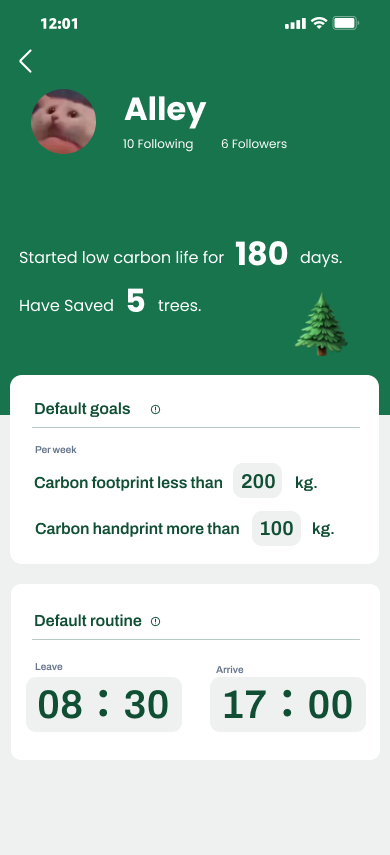
\includegraphics[width=0.3\columnwidth]{img/Default.png}
  \label{fig:Default}
  \caption{Default Screen}
\end{figure}


\section*{Discussion}

We believe that the derived design follows closely the design principles for visual design of user interfaces and Nielsen Design Principles.
Elements are grouped consistently, and the user interface can only be interpreted in one way. In a future design we would add also the financial savings achieved through the IoT Devices as it would be another gain for the user. Furthermore, the default screen design can be adapted to be exactly consisted with the Devices Screen, making it effortless to comprehend for users.
The largest limitation of the system is that it is currently only designed for a single user. This simplification of the design helped us to achieve a well-designed user interface, but limits the target customer group.





\bibliographystyle{apacite}
\bibliography{library}



\end{document}
